\documentclass[10pt, a4paper, spanish]{article}
\usepackage[paper=a4paper, left=1.5cm, right=1.5cm, bottom=1.5cm, top=3.5cm]{geometry}
\usepackage[utf8]{inputenc}
\usepackage[spanish]{babel}
\usepackage[autor]{caratula}
\usepackage[pdfencoding=auto, colorlinks=true, linkcolor=blue]{hyperref}
\usepackage[boxruled, longend]{algorithm2e}

\SetKwComment{Comment}{}{}
\SetKwInput{Pre}{Pre}
\SetKwInput{Post}{Post}

\newcommand\complejidad{\textbf{Complejidad}}
\newcommand\justifcomp{\textbf{Justificación}}
\newcommand\OdeLinea[1]{\Comment*[r]{$O(#1)$}}
\newcommand\OdeBloque[1]{\Comment*[f]{$O(#1)$}}

\newcommand{\TituloDis}[1]{
  \vspace*{1ex}\par\noindent\textbf{\large #1}\par
}

\newcommand{\algoritmo}[3]{\hangindent=\parindent#1 (#2) \ifx#3\empty\else$\rightarrow$ res: #3\fi}

\begin{document}

% CARATULA
\materia{Algoritmos y Estructuras de Datos III}
\submateria{Primer Cuatrimestre de 2017}
\fecha{\today}
\titulo{Trabajo Práctico 1}

\integrante{Tarrío, Ignacio}{363/15}{itarrio@dc.uba.ar}

\maketitle

\tableofcontents
\pagebreak

\section{Ejercicio 1 (BackTracking):}

En este ejercicio se nos pide resolver el problema utilizando un algoritmo de backtracking.

Backtracking es una técnica para buscar exhaustivamente todas las configuraciones del espacio de soluciones de un problema, para eso va generando las posibles soluciones constructivamente y va dejando atrás los candidatos cuando sabemos que no son válidos(que no pertenecen al espacio de soluciones válidas del problema).

Para este problema queremos buscar el minimo de numeros sin pintar para una secuencia de números de largo $n$. Ya que un número puede estar pintado de rojo, azul o sin pintar, y como tenemos $n$ números, podemos tener como máximo $3^n$ posibles combinaciones, aunque podrían ser menos ya que de esas combinaciones hay posibilidades que no son válidas como soluciones ya que puede ser que la subsecuencia de rojos no sea creciente o decreciente para la de azul. Una vez generadas todas estas soluciones, deberíamos encontrar la que menos numeros tiene sin pintar y esa va a ser la solución a nuestro problema(se nos pide la cantidad no qué combinación de rojos y azules).

Ya que estamos construyendo las distintas soluciones, empezamos decidiendo de qué color pintar el número primer número, rojo azul o sin pintar, para cada una de estas 3 decisiones vamos a pasar al siguiente número y repetir el proceso, así hasta llegar al final en el que vamos a tener como pintamos los numero y nos fijamos cuantos dejamos sin pintar. Una vez que tenemos todas las soluciones buscamos la óptima.

Se puede implementar este algoritmo de manera recursiva, dado el arreglo de números, el índice, y cuál fue el último rojo y último azul pintado(si hay), devuelve la mínima cantidad de números sin pintar dentro de las posibilidades. Pedimos el último rojo y el último azul porque no me importa saber cómo los pinte si no los últimos ya que eso me va a dar la limitante de si el próximo número lo puedo pintar de rojo o azul(y descartamos los que no pude pintar). Entonces esta función recursiva guarda los resultados del índice siguiente para las 3 posibilidades(rojo, azul y sin pintar), se fija cual es la menor y devuelve esa(si es la que no se pinta tiene que sumarle uno), excepto que sea el caso basó en el que no hay indice siguiente y devolvemos 0 si podemos pintarlo(0 elementos sin pintar en un arreglo que contiene sólo al último elemento pintado de cualquier color) o 1 si no lo pudimos pintar, y despues se van a ir llenando las anteriores llamadas con estos casos bases.

\subsection*{Pseudocodigo}
\begin{algorithm}[H]
\NoCaptionOfAlgo
	\KwData{	
	arreglo = el arreglo de numeros entero\\
	n = el tamaño del arreglo
	\KwResult{La cantidad minima de numeros sin pintar para una secuencia de numeros de largo n}
	\caption{\algoritmo{ej}{int arreglo[], n}{int}}
		\tcc{Empezamos el backtracking desde el primer indice(0) y no inicializamos todavia el ultimo rojo y el ultimo azul}
		res $\leftarrow$ BT(0, arreglo, n, NULL, NULL)\\
	}
\end{algorithm}
.\\
\begin{algorithm}[H]
\NoCaptionOfAlgo
	\KwData{
	i = indice actual a pintar\\
	arreglo = el arreglo de numeros entero\\
	n = el tamaño del arreglo\\
	ultimoRojo = el ultimo numero que se pinto de rojo(NULL si no se pinto ninguno)}
	\KwResult{La cantidad minima de numeros sin pintar a partir de i hasta n}
	\caption{\algoritmo{BT}{int i, arreglo[], n, ultimoRojo, ultimoAzul}{int}}

	numeroActual $\leftarrow$ arreglo[i]\\
	\eIf{ i = $n-1$ }{
		\tcc{Si el indice es el ultimo numero entonces estamos en el caso base}
		\tcc{Tenemos que fijarnos si podemos pintarlo}
		\eIf { ultimoRojo = NULL \textbf{or} ultimoAzul = NULL \textbf{or} ultimoRojo $<$ numeroActual \textbf{or} ultimoAzul $>$ numeroActual }{
			res  $\leftarrow$ 0
		}{
			\tcc{No lo podemos pintar porque no seria una solucion valida entonces devolvemos 1}
			res  $\leftarrow$ 1
		}
	}{	
		int minSiRojo, minSiAzul, minSinPintar\\
		\If{ ultimoRojo = NULL \textbf{or} ultimoRojo $<$ numeroActual} {
			\tcc{Si lo podemos pintar el numero actual de rojo osea si es mas grande que el anterior rojo pintado, o si es el primero rojo en pintarse, y cambiamos el ultimoRojo por este numero}
			minSiRojo $\leftarrow$ BT(i+1, arreglo, n, numeroActual, ultimoAzul)
		}
		\If{ ultimoAzul = NULL \textbf{or} numeroActual $<$ ultimoAzul} {
			\tcc{Lo mismo con el azul}
			minSiAzul $\leftarrow$ BT(i+1, arreglo, n, ultimoRojo, numeroActual)
		}
		\tcc{Calculamos tambien si no lo pintamos y al resultado le sumamos uno porque este no lo pintamos}
		minSinPintar $\leftarrow$ BT(i+1, arreglo, n, ultimoRojo, ultimoAzul) + 1\\
		\tcc{retornamos el minimo de ambos(considerando que la func min es O(1) y si es nulo la variable no lo considera)}
		res $\leftarrow$ min(minSiRojo, minSiAzul, minSinPintar)
	}

\end{algorithm}

\subsection*{Análisis de Complejidad}
Ya dijimos que la cantidad de combinaciones posibles son $3^n$, y podemos decir que este algoritmo recorre como máximo todas ellas porque empieza desde el índice 0 y por cada número del arreglo prueba las 3 combinaciones(nada más las válidas), entrando recursivamente al índice siguiente(i+1) y esos lo van a repetir hasta llegar al caso base que sería llegar al último índice. Ahora, cada llamada recursiva hace una cantidad de operaciones O(1) constantes (sumar, comparar, mínimo) y si no es el caso base además hace 3 llamadas recursivas en peor caso, pero reduciendo el n. Esto nos hace quedar que la complejidad de la función recursiva es $T(n) = 3T(n-1) + O(1)$ con $T(0) = 1$ como el caso base, que se puede demostrar fácilmente (por inducción) que es $O(3^n)$ para el peor caso. Otra forma de llegar es ver el árbol de ejecución de la recursión, cada nodo desprende tres nodos hijos, vamos a tener un árbol de altura n, y como es un árbol ternario tenemos $3^n$ hojas, que son nuestras soluciones. Esta complejidad se considera exponencial y es muy mala para instancias grandes.
Obviamente esto no pasa siempre, porque no siempre es posible entrar calcular las 3 posibilidades, de hecho es muy probable que no se pueda, supongamos que ya pintamos un numero de rojo y un número azul, para que entre a las tres bifurcaciones el número este tiene que ser mayor al rojo y menor al azul, osea que el azul tiene que ser mayor que el rojo y ademas el numero actual tiene que estar en el medio, ahora cuando sigamos con el próximo número esta brecha se va a haber achicado entonces va a ser menos probable que el número caiga en el medio de ambos.

\subsection*{Experimentación Computacional}
\subsubsection*{Instancias Aleatorias}
Se corrió una experimentación, sobre el código realizado en c++, generando arreglos aleatorios de tamaño n, y los números tienen una distribución uniforme donde el mínimo es 0 y el máximo es 2 veces n, esto se hizo así, para que exista una buena probabilidad de que haya números repetidos, ya que si por ejemplo hay un número repetido 3 veces no existe posibilidad de que el óptimo sea 0, así agregando casos malos a la experimentación. Se probaron arreglos de tamaño: 1, 2, 5, 10, 15, 20, 25, 30, 35. De cada uno de estos tamaños se computaron 30 arreglos diferentes, de estos 30 se tomo el promedio.

\begin{center}
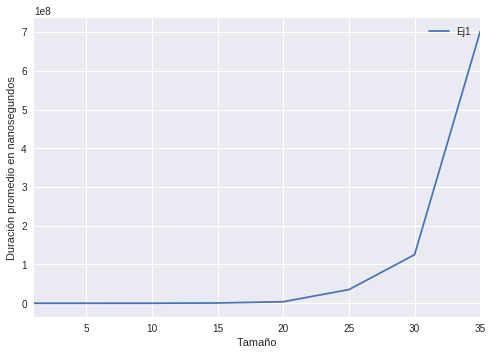
\includegraphics[scale=0.5]{ej1Random1-40.png}\\
\end{center}
Como podemos ver en el gráfico lo que tarda en resolver el problema aumenta exponencialmente a medida que crece el tamaño del arreglo, de hecho en promedio para calcular el arreglo de tamaño 35 es  0,701732075 segundos que es mucho, y para el de 30 tardó 0,125287312 segundos casi 5 veces más. Para seguir haciendo énfasis en que cada vez tarda más hagamos zoom para los primeros dato\\
\begin{center} 
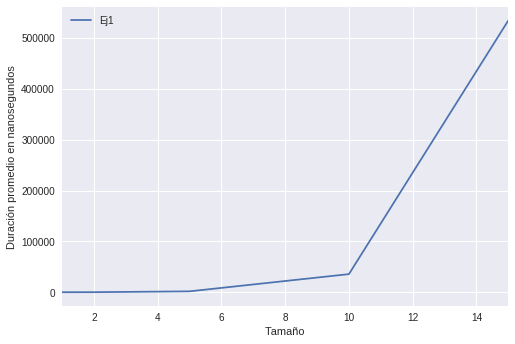
\includegraphics[scale=0.5]{ej1Random1-5.png}\\
\end{center}
En este gráfico también podemos apreciar como va creciendo exponencialmente(en el otro grafico parecia que al principio era constante la duración). En este caso tenemos que en promedio para los arreglos de tamaño 5 tardan 0,001741 milisegundos y para los de tamaño 10 tarda 0,035622 milisegundos casi 20 veces más.\\
Conclusión si bien es viable para instancias chicas, es muy ineficiente y tarda mucho cuando las instancias empiezan a ser más grande\\




\section{Ejercicio 2 (BackTracking con Poda):}

En este ejercicio nos piden hacer una mejora en el anterior algoritmo de backtracking y hacerle una poda. Las podas consisten en que hay instancias de soluciones parciales que ya no nos interesan y ni siquiera las calculamos, porque por ejemplo esta solucion va a hacer peor que una que ya calculamos anteriormente. Esto lo que provoca es una optimizacion porque dejamos de calcular cosas, aunque sigue siendo una busqueda exhaustiva.

Si recordamos el anterior algoritmo, para un indice calculaba el menor si lo pintabamos de rojo, despues de azul y despues sin pintar, pero que pasa si uno nos devuelve que se pueden pintar todos los proximos numeros, osea que los los otros no hace falta computarlos ya que solo nos importa la cantidad de numeros sin pintar, y no vamos a encontrar una mejor porque esta es la minima. Esta es nuestra primer poda, una vez calculado una solucion parcial para un color, nos fijamos si es optima y si lo es nos salteamos(no computamos) las otras alternativas de colores.	Tambien podriamos llevar una cuenta de cual es la solucion(entera) optima y no calculamos una que pueda ser peor que esa, por ejemplo si voy por el 3 indice y encontramos una solucion que solo no puede pintar un numero, solo tenemos que buscar una solucion que pinta todos los numeros, asi que no vamos a entrar a las recursiones de no pintar.

Para la implementacion de estas podas modificamos un poco la base del codigo del anterior ejercicio asi se nos es mas facil calcular los datos. Ahora la funcion recursiva tiene 2 parametros de entrada nuevos, el minimo encontrado en las soluciones ya calculadas y la cantidad de numeros que ya no pintamos y ahora en vez de devolver un resultado parcial, devuelve la cantidad de sin pintar para todo el arreglo(ya que tenemos la cantidad que no pintamos antes).

Pseudocodigo:

\begin{algorithm}[H]
\NoCaptionOfAlgo
	\KwData{	
	arreglo = el arreglo de numeros entero\\
	n = el tamaño del arreglo
	\KwResult{La cantidad minima de numeros sin pintar para una secuencia de numeros de largo n}
	\caption{\algoritmo{ej2}{int arreglo[], n}{int}}
		\tcc{Empezamos el backtracking desde el primer indice(0) y no inicializamos todavia el ultimo rojo y el ultimo azul, y ademas por defecto el optimo es n(no existe peor solucion que esta) y no pintamos ninguno todavia}
		res $\leftarrow$ BT(0, arreglo, n, NULL, NULL, n, 0)\\
	}
\end{algorithm}

\begin{algorithm}[H]
	\NoCaptionOfAlgo
	\KwData{
	i = indice actual a pintar\\
	arreglo = el arreglo de numeros entero\\
	n = el tamaño del arreglo\\
	ultimoRojo = el ultimo numero que se pinto de rojo(NULL si no se pinto ninguno)}
	ultimoAzul = el ultimo azul pintado\\
	optimoActual = la mejor solucion encontrada hasta el momento
	sinPintar = cantidad de numeros sin pintar antes de i\\
	\KwResult{La cantidad minima de numeros sin pintar a partir de i hasta n}
	\caption{\algoritmo{BTI}{int i, arreglo[], n, ultimoRojo, ultimoAzul, optimoActual, sinPintar}{int}}

	numeroActual $\leftarrow$ arreglo[i]\\
	\eIf{ i = $n-1$ }{
		\tcc{Si el indice es el ultimo numero entonces estamos en el caso base}
		\tcc{Tenemos que fijarnos si podemos pintarlo}
		\eIf { ultimoRojo = NULL \textbf{or} ultimoAzul = NULL \textbf{or} ultimoRojo $<$ numeroActual \textbf{or} ultimoAzul $>$ numeroActual }{
			res  $\leftarrow$ sinPintar
		}{
			\tcc{No lo podemos pintar porque no seria una solucion valida entonces devolvemos la cantidad que pintamos antes mas 1 porque este no lo pintamos}
			res  $\leftarrow$ sinPintar + 1
		}
	}{	
		int minSiRojo, minSiAzul, minSinPintar\\
		\If{ ultimoRojo = NULL \textbf{or} ultimoRojo $<$ numeroActual} {
			minSiRojo $\leftarrow$ BTI(i+1, arreglo, n, numeroActual, ultimoAzul, optimoActual, sinPintar)\\
			\tcc{PODA 1: si es el optimo no calculamos los demas y devolvemos este}
			\If{minSiRojo $=$ sinPintar}{
				res $\leftarrow$ minSiRojo
			}
			\If{ minSiRojo $<$ sinPintar} {
				optimoActual $\leftarrow$ minSiRojo
			}
		}
		\If{ ultimoAzul = NULL \textbf{or} numeroActual $<$ ultimoAzul} {
			\tcc{Lo mismo con el azul}
			minSiAzul $\leftarrow$ BTI(i+1, arreglo, n, ultimoRojo, numeroActual, optimoActual, sinPintar)\\
			\tcc{PODA 1}
			\If{minSiAzul $=$ sinPintar}{
				res $\leftarrow$ minSiAzul
			}
			\If{ minSiAzul $<$ sinPintar} {
				optimoActual $\leftarrow$ minSiAzul
			}
		}
		\tcc{PODA 2: solo calculamos sin pintar este numero, si todavia podemos mejorar el optimo}
		\If{sinPintar $<$ optimoActual $- 1$} {
			minSinPintar $\leftarrow$ BTI(i+1, arreglo, n, ultimoRojo, ultimoAzul, optimoActual, sinPintar + 1)\\
		}
		res $\leftarrow$ min(minSiRojo, minSiAzul, minSinPintar)
	}

\end{algorithm}

Podemos apreciar que en el peor de los casos tenemos que seguir calculando los 3 caminos asi que no podemos mejorar la complejidad. Pero sin embargo vamos a recortar muchas ramas, que no necesitamos calcular, ya que por ejemplo si encontramos el optimo pintando de rojo nos ahorramos 2/3 de las difurcaciones al no calcular si pintamos de azul y si no lo pintamos y ademas si estamos al limite de numeros sin pintar comparados con el optimo no avanzamos en las ramas de no pintar.

El algoritmo es correcto ya que las soluciones que descartamos sabemos que son peores a las que ya calculamos.

   





\section{Ejercicio 3 (Programacion dinamica):}
La programación dinamica es otra tecnica algoritmica, consiste en resolver los subproblemas de tamaños menores y dados estos resultados, generar la solución al problema original, pero la tecnica aprovecha estructuras de datos(generalmente matrices) para guardar los subproblemas que ya calculamos, y si en algun momento lo tenemos que calcular de nuevo(por ejemplo si dos subproblemas del mismo tamaño necesitan del mismo subproblema de tamaño mas chico) nos ahorramos el calculo porque tenemos en la estructura con la respuesta.


Principio de optimalidad de Bellman:
Un problema satisface el principio si una subsolucion optima debe ser solucion del subproblema asociado a esa subsolucion. En este problema podriamos decir que para una secuencia de largo n un subproblema sea la subsecuencia de 0 a n - 1, y si tenemos esta subsolucion, entonces, la solucion al problema original va a ser menor o igual a esta subsolucion, de hecho va a ser igual o la misma menos uno(siempre y cuando no sea 0). Probemos esto que acabamos de decir, supongamos que tenemos una subsolucion que vale $x \geq 2$ para el subproblema de tamaño igual menos uno a la del problema que tenemos que resolver, y tambien supongamos que la solucion al problema es un $x'$ tal que $x' = x - 2$, si pasa esto podriamos quedarnos con esa combinacion de colores(con la que nos da $x'$) sacarle el ultimo numero y tendriamos una nueva respuesta $x''$ tal que $x'' = x'-1$ ya que solamente sacamos el ultimo numero, pero entonces $x'' < x$ osea que $x$ no era optima, por ende entramos en un absurdo. Que esto lo supusimos al decir que habia una solucion mucho mejor que la de la solucion. Osea que de una subsolucion no podemos empeorar la solucion o solo la empeoramos en una unidad, la dejamos igual cuando el nuevo numero lo podemos pintar desde alguna de la combinaciones optimas anteriores, o empeora en uno si no existe combinacion optima anterior desde la cual no podamos pintar este numero de rojo o de azul(notar que ahora hay combinaciones que por ahi no son optimas para el subproblema anterior pero se diferencian en uno). Gracias a esto cumple el principio de optimalidad de Bellman, pero notemos que si el problema fuese dar las subsecuencias rojas y azules, no se cumpliria el principio ya que, por lo ultimo que dijimos, cuando no hay una combinacion optima anterior puede ser que las nuevas soluciones no esten asociadas a las del subproblema, entonces no cumpliria el principio.

Como vimos en backtracking al pintar un numero, solo nos importa cuales fueron el ultimo rojo y el ultimo azul que se pintaron, entonces al agregar un nuevo a la secuencia, tenemos que buscar la combinacion de ultimo rojo y ultimo azul optima tal que nos deje pintar este ultimo numero o buscar una combinacion de rojo y azul la cual no pintemos este ultimo pero sea mejor que si lo pintaramos. Entonces por problema tenemos que buscar cual es la combinacion de ultimo rojo y ultimo azul que nos haga optima la solucion.

El algoritmo dado se va a basar en eso, va a terminar calculando todas las combinaciones de ultimo rojo y ultimo azul para ver cual es la optima. Como calculamos cada una de estas combinaciones? recientemente dijimos que para pintar un numero de forma optima teniamos que buscar en la combinacion de ultimo rojo ultimo azul valida que sea optima. Entonces si queremos pintar el ultimo indice de rojo, sea $r$, y como ultimo azul un indice $a$ con $0 \leq a < r$, deberiamos buscar el $r'$ tal que sea optimo y que $secuencia_{r'} < secuencia_r$, para esto vamos a tener que recorrer de $0$ a $r-1$ buscando el que cumpla estas condiciones.
Otro tema importante de la programacion dinamica es como guardamos los datos, una manera es tener una matriz de 2 dimensiones, en el que el indice de la fila representa el indice del ultimo azul y el indice de la columnas el del rojo, osea que sea $M$ la matriz, $M_{r,b}$ nos da cual la subsolucion para esa combinacion de rojo y azul. Un caso que deje afuera pero hay que tener en cuenta es que hay una combinacion que es en la que no se pinta ninguno de rojo o de azul, o no se pinta ninguno, este indice se va a representar en la ultima fila y en la ultima columna, resumiendo para un problema de $n$ numeros vamos a tener una matriz $M$ de ($n+1 x n+1$) donde la la fila n+1 y la columna n+1 representan cuando el ultimo azul o ultimo rojo respectivamente son nulos.

Este es nuestro algoritmo, calculamos la matriz y buscamos en ella cual es el optimo, ahora tenemos que decidir en que orden calculamos los datos, ya que como para calcular $M_{r,b}$ tenemos que tener calculado $M_{i,b}$ con $i<r$ y $M_{r+1,b}$ va a necesitar de estos tambien, podemos ir de una manera constructiva, empezando en los casos bases, que son los cuando pintamos nada mas el primero de un color(que sabemos que va a dejar a todos los otros numeros siguientes sin pintar entonces la subsolucion es n - 1) y si no pintamos ninguno(osea quedan n sin pintar), esto era el indice 0, despues pasamos para el indice 1 y calculamos todas las combinaciones nuevas, osea ya teniamos calculado $M_{0,n+1}$ y $M_{n+1,0}$ y $M_{n+1,n+1}$, y ahora calculamos $M_{1,0}$, $M_{1,n+1}$, $M_{0,1}$, $M_{n+1, 1}$ (notar que $M_{r,b}$ con $r = b$ es invalido porque no podemos pintar un mismo numero de dos colores). Una vez calculada toda la matriz buscamos el optimo dentro de esta y esa es nuestra solucion.


\begin{algorithm}[H]
\NoCaptionOfAlgo
	\KwData{	
	arreglo = el arreglo de numeros entero\\
	n = el tamaño del arreglo\\
	\KwResult{La cantidad minima de numeros sin pintar para una secuencia de numeros de largo n}
	\caption{\algoritmo{ej3}{int arreglo[], n}{int}}
		\tcc{Creamos nuestra matriz}
		int m[n+1][n+1]\\ \\

		\tcc{Le guardamos los triviales, los del primer indice(0)}
		int m[0][n] = n - 1\\
		int m[n][0] = n - 1\\
		int m[n][n] = n \\ \\
		res $\leftarrow$ BT(0, arreglo, n, NULL, NULL, n, 0)\\

		\tcc{Ahora recorremos todos los indices}
		\For(){$i \leftarrow 1$ \KwTo n}{
			\tcc{Y para cada indice, calculamos el optimo si pintaramos este de azul o de rojo y las combinaciones del otro}
			\For(){$j \leftarrow o$ \KwTo i - 1}{
				m[i][j] $\leftarrow$ buscarOptimoPintandoDeRojo(i, j, arreglo, m, n) \\
				m[j][i] $\leftarrow$ buscarOptimoPintandoDeAzul(i, j, arreglo, m, n)
			}
			\\
			\tcc{En esa iteracion dejamos de lado la combinacion si pintamos este ultimo de azul y no pintamos ninguno de rojo, y viceversa}
			m[i][n] $\leftarrow$ buscarOptimoPintandoDeRojo(i, n, arreglo, m, n) \\
			m[n][i] $\leftarrow$ buscarOptimoPintandoDeAzul(i, n, arreglo, m, n)
		}

		\tcc{Una vez ya calculada la matriz buscamos el menor, min es una funcion que busca el menor de una matriz en $O(m)$ donde m es la cantidad de elementos que hay en la matriz}
		res $\leftarrow$ min(m)
	}
\end{algorithm}

\begin{algorithm}[H]
\NoCaptionOfAlgo
	\KwData{	
	r = El indice que estamos pintando de rojo\\
	a = El indice que fijamos de azul\\
	arreglo = La secuencia de numeros \\
	m = La matriz(pasa por referencia)\\
	n = el tamaño del arreglo\\
	\KwResult{La cantidad minima de numeros sin pintar si elejimos como ultimo pintado de rojo al indice r y de azul a a}
	\caption{\algoritmo{buscarOptimoPintandoDeRojo}{int r, a, arreglo[], m, n}{int}}
		\tcc{Ponemos como optimo momentaneo al $M_{n, a}$ osea si el primer rojo que pintamos sea este numero, total siempre es una solucion valida}
		int optimoActual $\leftarrow$ m[n][a]\\
		\tcc{Recorremos con el azul fijado, que pasaria si partieramos desde los anteriores rojos}
		\For(){$ri \leftarrow 0$ \KwTo r - 1}{
			\tcc{Nos fijamos si el numero de la secuencia de ri es menor al de r,(osea si podemos pintarlo a partir de ri), y si es mas chico que el optimoActual}
			\If{ri != a \textbf{and} arreglo[ri] $<$ arreglo[r] \textbf{and} m[ri][a] $<$ optimoActual}{
				\tcc{Si es menor, marcamos a este como el optimoActual}
				optimoActual $\leftarrow$ m[ri][a]
			}
		}
		\tcc{Retornamos el optimo del cual podemos pintar y como pintamos este ultimo se reduce en 1}
		res $\leftarrow$ optimoActual - 1 
	}
\end{algorithm}

\begin{algorithm}[H]
\NoCaptionOfAlgo
	\KwData{	
	a = El indice que estamos pintando de azul\\
	r = El indice que fijamos de rojo\\
	\caption{\algoritmo{buscarOptimoPintandoDeRojo}{int a, j, arreglo[], m, n}{int}}
		\tcc{El codigo de esta funcion es totalmente analogo al de rojo}
		int optimoActual $\leftarrow$ m[r][n]\\
		\For(){$ai \leftarrow 0$ \KwTo a - 1}{
			\If{ai != r \textbf{and} arreglo[ai] $>$ arreglo[a] \textbf{and} m[r][ai] $<$ optimoActual}{
				optimoActual $\leftarrow$ m[r][ai]
			}
		}
		res $\leftarrow$ optimoActual - 1 
	}
\end{algorithm}

\subsection*{Analisis de Complejidad}
Vamos a calcular en todos los casos, toda la matriz que ambas dimensiones son de tamaños $n+1$, osea que ya recorrer todos los elementos nos cuesta $O(n^2)$ y para calcular cada una de estos elementos de la matriz recorremos $O(n)$ elementos(en la funcion auxiliar para buscar el optimo), eso ya nos da una complejidad de $O(n^3)$ y despues buscar el optimo dentro de la matriz tambien es $O(n^2)$ y despues son una cantidad constante de operaciones elementales, en definitiva nos queda una complejidad para el peor de los casos de $O(n^3)$, de hecho en el codigo dado no cortamos nunca y siempre completamos la matriz entonces para cualquier caso el codigo va a hacer $O(n^3)$. Una alternativa de analisis es considerar los casos que tenemos, podriamos decir que tenemos 3 variables en cada caso, el ultimo azul, el ultimo rojo, y el indice, entonces como cada una de estas variables esta acotada por $n$ tenemos $n^3$ casos y son los que terminamos calculando.



\end{document}